\documentclass{standalone}
%outline around text
\usepackage[outline]{contour}
\contourlength{1.3pt}

%tikz
\usepackage{tikz}
\usetikzlibrary{knots, cd, calc}

\begin{document}
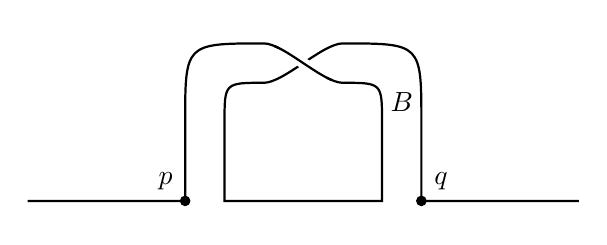
\begin{tikzpicture}
\begin{knot}[clip width = 5, consider self intersections = true]
\clip (2, -0.2) rectangle (9, 2.2);
\strand[thick] (2, 0) -- (4, 0) -- (4, 1)
				.. controls +(0, 1) and +(-1, 0) .. (5, 2)
				.. controls +(0.25, 0) and +(-0.25, 0) .. (6, 1.5)
				.. controls +(0.5, 0) and +(0, 0.5) .. (6.5, 1)
				-- (6.5, 0) -- (4.5, 0) -- (4.5, 1)
				.. controls +(0, 0.5) and +(-0.5, 0) .. (5, 1.5)
				.. controls +(0.25, 0) and +(-0.25, 0) .. (6, 2)
				.. controls +(1, 0) and +(0, 1) .. (7, 1)
				-- (7, 0) -- (9, 0);
\end{knot}
\node at (3.75, 0.25) {\contour{white}{$p$}};
\node at (7.25, 0.25) {\contour{white}{$q$}};
\node at (6.75, 1.25) {$B$};
\draw[fill = black] (4, 0) circle (0.06);
\draw[fill = black] (7, 0) circle (0.06);
\end{tikzpicture}
\end{document}